\chapter{Lezione 6}
\label{chap:lezione_06} 

\begin{flushright}
\textit{Data: 13/10/2025}
\end{flushright}


\section{Stato e Fase}

L'idea di \textbf{stato} del sistema è legata a come il sistema si trova in un dato istante di tempo fisico all'equilibrio. È una definizione molto precisa.

Generalmente, si inizia preparando il sistema. Tipicamente, il sistema sarà fuori equilibrio, quindi lo si lascia evolvere per un certo periodo fino a quando non raggiunge l'equilibrio. In una simulazione Monte Carlo, ad esempio, si parte da un punto e si lascia evolvere. Da un certo momento in poi, il sistema sarà all'equilibrio. Questo significa che si avrà un insieme di configurazioni. Ad esempio, le molecole e l'aria in questa stanza: le molecole in equilibrio evolvono passando attraverso diverse configurazioni, ma in modo tale che le quantità misurabili rimangano costanti.

L'insieme delle configurazioni che appare tipicamente in un dato istante di tempo è lo stato del sistema.

\vspace{0.5cm}

\textbf{Distinzione tra Stato e Fase:}
\begin{itemize}
    \item \textbf{Stato:} In questo contesto, lo stato è utilizzato come \textbf{gruppo di configurazioni} che appaiono fisicamente in un momento. Ad esempio, la configurazione delle molecole cambia in un secondo, ma è "equivalente" a quella precedente.
    
    Lo \textbf{stato è puro quando coincide con la realizzazione fisica del sistema}. Si identifica lo stato puro con il \textbf{comportamento a tempi lunghi di un singolo sistema}.

    \item \textbf{Fase:} Si usa il concetto di fase per \textbf{distinguere due regimi diversi caratterizzati da parametri differenti}. Ad esempio, per distinguere un sistema magnetizzato da uno non magnetizzato.
\end{itemize}



\begin{enumerate}
    \item Per $T$ grande ($T \gg T_c$), lo stato puro è lo stato con magnetizzazione zero $\langle\cdot\rangle_{0}$
    \item Per $T$ piccola ($T < T_c$), lo stato simmetrico ($m=0$) non è puro, perché all'equilibrio non si osserva mai lo stato con magnetizzazione zero. Lo stato è una \textbf{miscela statistica} degli stati puri $\langle\cdot\rangle_{+}$ e $\langle\cdot\rangle_{-}$
\end{enumerate}



\section{Rottura Spontanea di Simmetria}

\begin{tcolorbox}[colback=yellow!30,  
                  colframe=yellow!50!orange,  
                  boxrule=0.8pt, 
                  arc=3pt,  
                  top=4pt, bottom=4pt, left=6pt, right=6pt,
                  enhanced,
                  sharp corners=south]
\textbf{Un gruppo di simmetria $G$ è spontaneamente rotto se lo stato simmetrico (con $m=0$) non è puro e può essere scomposto come combinazione convessa di stati puri che si trasformano come una rappresentazione non-banale di $G$}.
\end{tcolorbox} 


Nel caso semplice di magnetizzazione, una rappresentazione non-banale è quella che ha \textbf{magnetizzazione non-zero}.

Se si ha un campo magnetico ($h \ne 0$), la simmetria è \textbf{rotta esplicitamente}.



\section{Proprietà di Clustering}

Consideriamo sistemi omogenei con un'Hamiltoniana $H$. Si aggiunge una perturbazione localizzata $\delta H$ vicino al punto $x$:
\begin{equation}
\delta H = P(x) \label{eq:perturbation}
\end{equation}

\begin{tcolorbox}[colback=yellow!30,  
                  colframe=yellow!50!orange,  
                  boxrule=0.8pt, 
                  arc=3pt,  
                  top=4pt, bottom=4pt, left=6pt, right=6pt,
                  enhanced,
                  sharp corners=south]
\noindent Se si misura il valore di aspettazione di un'osservabile $A(y)$ lontano dal punto $x$, ci si aspetta che non cambi significativamente:
\begin{equation}
\langle A(y) \rangle \text{ non cambia per } |x-y| \rightarrow \infty \label{eq:clustering_intuition}
\end{equation}
La \textbf{teoria della risposta lineare} (Linear Response Theory) stabilisce che questo accade se:
\begin{equation}
C^c[P(x), A(y)] = \langle P(x) A(y) \rangle - \langle P(x) \rangle \langle A(y) \rangle \xrightarrow{|x-y| \rightarrow \infty} 0 \quad \forall A, P \label{eq:clustering_condition}
\end{equation}

\noindent Questa proprietà è chiamata \textbf{proprietà di clustering}.


\noindent Se la proprietà di clustering è valida per un dato stato, \textbf{lo stato è chiamato "clustering"}.
\end{tcolorbox} 

%Sotto la temperatura critica ($T < T_c$), il sistema sviluppa una magnetizzazione spontanea non nulla, $m = |\langle \sigma_i \rangle| > 0$. begin{itemize} \item \textbf{Stati Puri $\langle\cdot\rangle_{\pm}$ :} Nello stato $\langle\cdot\rangle_{+}$, la magnetizzazione è $\langle\sigma_i\rangle_{+} = m$. Se lo stato è puro deve essere di clustering, e il valore di aspettazione del prodotto a grande distanza è: $$ \langle\sigma_i \sigma_j\rangle_{+} \xrightarrow{|i-j| \rightarrow \infty} \langle\sigma_i\rangle_{+} \langle\sigma_j\rangle_{+} = m^2 $$La funzione di correlazione connessa è quindi:$$ C_{+}^c(i, j) = \langle\sigma_i \sigma_j\rangle_{+} - \langle\sigma_i\rangle_{+} \langle\sigma_j\rangle_{+} \xrightarrow{|i-j| \rightarrow \infty} m^2 - m^2 = 0 $$Poiché la correlazione connessa si annulla, lo stato $\langle\cdot\rangle_{+}$ (idem per lo stato $\langle\cdot\rangle_{-}$) è uno \textbf{stato clustering}.\item \textbf{Stato Simmetrico $\langle\cdot\rangle_{0}$ :}Il valore di aspettazione della magnetizzazione è zero: $\langle\sigma_i\rangle_{0} = \frac{1}{2}(m + (-m)) = 0$. Il valore di aspettazione del prodotto $\langle\sigma_i \sigma_j\rangle_{0}$ per $|i-j| \rightarrow \infty$ è (usando il risultato degli stati puri):\begin{equation}\langle\sigma_i \sigma_j\rangle_{0} \xrightarrow{|i-j| \rightarrow \infty} \frac{1}{2} (\langle\sigma_i \sigma_j\rangle_{+} + \langle\sigma_i \sigma_j\rangle_{-}) \xrightarrow{|i-j| \rightarrow \infty} \frac{1}{2} (m^2 + (-m)^2) = m^2 \ne 0\end{equation} La funzione di correlazione connessa è:\begin{equation}C_{0}^c(i, j) = \langle\sigma_i \sigma_j\rangle_{0} - \langle\sigma_i\rangle_{0} \langle\sigma_j\rangle_{0} \xrightarrow{|i-j| \rightarrow \infty} m^2 - (0)(0) = m^2\end{equation}Poiché $C_{0}^c(i, j)$ non si annulla a grande distanza, questo stato \textbf{non è clustering}. Le correlazioni non decadono. Nonostante la magnetizzazione media sia zero, gli spin sono \textbf{correlati positivamente} a distanza infinita. Se in un punto si trova uno spin positivo, è probabile che anche uno spin molto lontano sia positivo, poiché l'intero sistema è forzato a trovarsi in uno dei due stati puri ($\langle\cdot\rangle_{+}$ o $\langle\cdot\rangle_{-}$) per tempi estremamente lunghi. \end{itemize}

Al di sotto della temperatura critica ($T < T_c$), il sistema di Ising presenta una rottura spontanea di simmetria e ammette due tipi fondamentali di stati.

\begin{itemize}
    \item \textbf{Stati Puri}: $\langle\cdot\rangle_{+}$ e $\langle\cdot\rangle_{-}$
    
     Sono \textbf{stati clustering}. La funzione di correlazione connessa decade esponenzialmente a zero per grande distanza. L'influenza di uno spin è limitata a una lunghezza di correlazione finita ($\xi < \infty$). Due spin molto distanti sono statisticamente indipendenti.


    \item \textbf{Stato Simmetrico}: $\langle\cdot\rangle_{0}$
    
     \textbf{Non è uno stato clustering}. La correlazione connessa non si annulla a grande distanza, ma tende al valore costante $m^2 \ne 0$. Questo implica che gli spin rimangono \textbf{correlati positivamente} su distanze infinite, riflettendo la natura non-locale dello stato.
   
\end{itemize}

\vspace{0.5cm}


\section{Modello di Ising e Approssimazione di Campo Medio}

Si considerano \textbf{sistemi magnetici}. Il comportamento del sistema al punto critico è determinato solo da pochi elementi cruciali della Hamiltoniana (principio di \textbf{universalità}). Questi elementi sono:
\begin{enumerate}
    \item La \textbf{dimensionalità} del sistema ($D$ e la dimensionalità interna)
    \item Le \textbf{simmetrie} della Hamiltoniana
    \item Il \textbf{tipo di variabili} utilizzate (scalari, vettoriali, binarie, continue, ecc.)
\end{enumerate}

Nel \textbf{modello di Ising}, le variabili di spin sono binarie:
\begin{equation}
S_i = \pm 1
\end{equation}
Nel \textbf{modello di Heisenberg}, lo spin ha 3 componenti sulla sfera unitaria:
$$ \sum_{\nu=1}^{3} (S_i^{\nu})^2 = 1 \quad \forall i $$

L'Hamiltoniana esplicita per il \textbf{modello di Ising} è:
\begin{equation}
H_{I} = -J \sum_{\langle i, k \rangle} S_i S_k - \sum_{i} h_i S_i
\end{equation}
Dove $\langle i, k \rangle$ indica la somma sui primi vicini.

\begin{itemize}
    \item Se $J > 0$ (\textbf{ferromagnete}): Gli spin tendono ad essere \textbf{paralleli}.
    \item Se $J < 0$ (\textbf{antiferromagnete}): Gli spin tendono ad essere \textbf{antiparalleli}.
\end{itemize}

\vspace{0.5cm}


Se $J < 0$ e il sistema è su un \textbf{reticolo triangolare}, il sistema è \textbf{frustrato}: non è possibile minimizzare l'energia simultaneamente per tutti i legami.
\begin{itemize}
    \item La migliore energia che si può ottenere per un triangolo è $-J$ (non $-3J$), perché si soddisfano solo due legami su tre.
    \item La \textbf{frustrazione causa degenerazione} dello stato fondamentale. Ci sono più configurazioni che portano all'energia minima.
\end{itemize}

\newpage
\subsubsection{Approssimazione di Campo Medio}

In 3 dimensioni ($D=3$), il modello non è risolvibile.
L'\textbf{Approssimazione di Campo Medio} cerca di trovare la distribuzione di probabilità che minimizza l'energia libera di Helmholtz $F$:
\begin{equation}
F[P] = E[P] - \frac{1}{\beta} S[P] \label{eq:free_energy_functional}
\end{equation}
Dove $E[P]$ è l'energia media e $S[P]$ è l'entropia:
\begin{align*}
E[P] &= \langle H \rangle_P \\
S[P] &= -\int [ds] P[s] \log P[s]
\end{align*}
Si sa che la distribuzione di equilibrio è della forma $P_{eq} \propto e^{-\beta H}$.

\begin{tcolorbox}[colback=red!20,  
                  colframe=red!50!orange,  
                  boxrule=0.8pt, 
                  arc=3pt,  
                  top=4pt, bottom=4pt, left=6pt, right=6pt,
                  enhanced,
                  sharp corners=south]
\noindent \textbf{Ipotesi dell'Approssimazione di Campo Medio:} 

La probabilità è fattorizzata sui siti del reticolo.
\begin{equation}
P[\sigma] = \prod_{i=1}^{N} P_i(\sigma_i) \label{eq:mean_field_hp}
\end{equation}
\end{tcolorbox} 



Questa è un'approssimazione molto forte, in quanto implica che \textbf{ciò che accade su un sito non è realmente connesso a ciò che accade su un altro}.

La distribuzione di probabilità sul singolo sito $i$ è parametrizzata:
\begin{equation}
P_i(\sigma_i) = \delta_{\sigma_i=+1} \frac{1+m_i}{2} + \delta_{\sigma_i=-1} \frac{1-m_i}{2}
\end{equation}
I parametri $\{m_i\}$ dipendono dal sito.

\vspace{0.5cm}

\noindent \textbf{Proprietà della Distribuzione Fattorizzata:}

\begin{itemize}
    \item \textbf{Normalizzazione:}
    \begin{equation}
        \sum_{\sigma_i=\pm 1} P_i(\sigma_i) = \frac{1+m_i}{2} + \frac{1-m_i}{2} = 1
    \end{equation}  
    
    \begin{equation}
        \sum_{\sigma_1 \cdots \sigma_N} P[\sigma] = \prod_i \sum_{\sigma_i} P_i(\sigma_i) = 1^N = 1
    \end{equation} 
    \item \textbf{Magnetizzazione Media sul Sito:}
    Il parametro $m_i$ è il valore di aspettazione dello spin sul sito $i$:
    \begin{align}
    \langle\sigma_i\rangle &=  \sum_{\sigma_i=\pm 1} P_i(\sigma_i) \sigma_i \\
    &= \frac{1+m_i}{2}(+1) + \frac{1-m_i}{2}(-1) \\
    &= \frac{1+m_i - (1-m_i)}{2} = \frac{2m_i}{2} = m_i
    \end{align}
    \item \textbf{Valore di Aspettazione di una Funzione Generica $g(\sigma_i)$:}
    \begin{align}
    \langle g(\sigma_i) \rangle &=  \underbrace{\left( \sum_{\sigma_{j \neq i }=\pm 1} P_j(\sigma_j) \right)}_{ 1^{N-1}} \sum_{\sigma_i=\pm 1} P_i(\sigma_i) g(\sigma_i) \\ &= \frac{1+m_i}{2} g(+1) + \frac{1-m_i}{2} g(-1) \label{eq:generic_exp_val}
    \end{align}
\end{itemize}

\vspace{0.5cm}

\subsubsection{Calcolo dell'Energia Media :}
L'energia media è:
\begin{equation}
U = \langle H \rangle_P = \left\langle -J \sum_{\langle i, k \rangle} \sigma_i \sigma_k \right\rangle_P - \left\langle \sum_{i} h_i \sigma_i \right\rangle_P
\end{equation}
Grazie all'ipotesi di fattorizzazione della probabilità ($P[\sigma] = \prod_i P_i(\sigma_i)$):
$$ \langle \sigma_i \sigma_k \rangle = \langle \sigma_i \rangle \langle \sigma_k \rangle = m_i m_k \quad \text{per } i \ne k $$
Quindi l'energia media diventa:
\begin{equation}
U = -J \sum_{\langle i, k \rangle} m_i m_k - \sum_{i} h_i m_i \label{eq:mean_energy}
\end{equation}

\vspace{0.5cm}

\subsubsection{Calcolo dell'Entropia:}
L'entropia è data da:
\begin{equation}
S = -\sum_{i} \langle \log P_i(\sigma_i) \rangle = -\sum_{i} \sum_{\sigma_i=\pm 1} P_i(\sigma_i) \log P_i(\sigma_i)
\end{equation}
Sostituendo $P_i(\pm 1) = \frac{1 \pm m_i}{2}$:
\begin{equation}
S = -\sum_{i} \left\{ \frac{1+m_i}{2} \log\left(\frac{1+m_i}{2}\right) + \frac{1-m_i}{2} \log\left(\frac{1-m_i}{2}\right) \right\} \label{eq:mean_field_entropy}
\end{equation}

\vspace{0.5cm}

\subsubsection{Energia Libera e Condizione di Equilibrio:}
L'energia libera è:
\begin{equation}
F = U - \frac{1}{\beta} S \label{eq:mean_field_free_energy}
\end{equation}
I parametri $\{m_i\}$ (che sono i valori di aspettazione $\langle\sigma_i\rangle$) sono determinati minimizzando l'energia libera, che in questo caso è una funzione (non un funzionale) dei parametri $m_i$.

Cerchiamo i punti stazionari dell'energia libera:
\begin{equation}
\frac{\partial F}{\partial m_i} = 0 \quad \forall i
\end{equation}
Per garantire un minimo di equilibrio, si deve controllare la derivata seconda:
\begin{equation}
\frac{\partial^2 F}{\partial m_i^2} > 0
\end{equation}
Questo sarà cruciale per determinare la \textbf{transizione di fase}. 

L'analisi di $F(m)$ permette di determinare la stabilità delle soluzioni:
\begin{itemize}
    \item $T > T_c$: $F(m)$ ha un solo minimo in $m=0$
    
    \item $T = T_c$:  Il minimo in $m=0$ diventa molto piatto. Sia la derivata prima che la derivata seconda sono zero in $m=0$. 

    \item $T < T_c$: La forma della funzione cambia in una "doppia buca" (double well). Ci sono due minimi simmetrici in $m^\pm$, che sono le soluzioni stabili. Il punto $m=0$ è ora un massimo locale, che corrisponde a una soluzione instabile. 
    
\end{itemize}


\begin{figure}[h!]
    \centering
    \begin{minipage}[b]{0.4\textwidth}
        \centering
        \includegraphics[width=\textwidth]{pics/03.png}
    \end{minipage}
    \hfill
    \begin{minipage}[b]{0.4\textwidth}
        \centering
        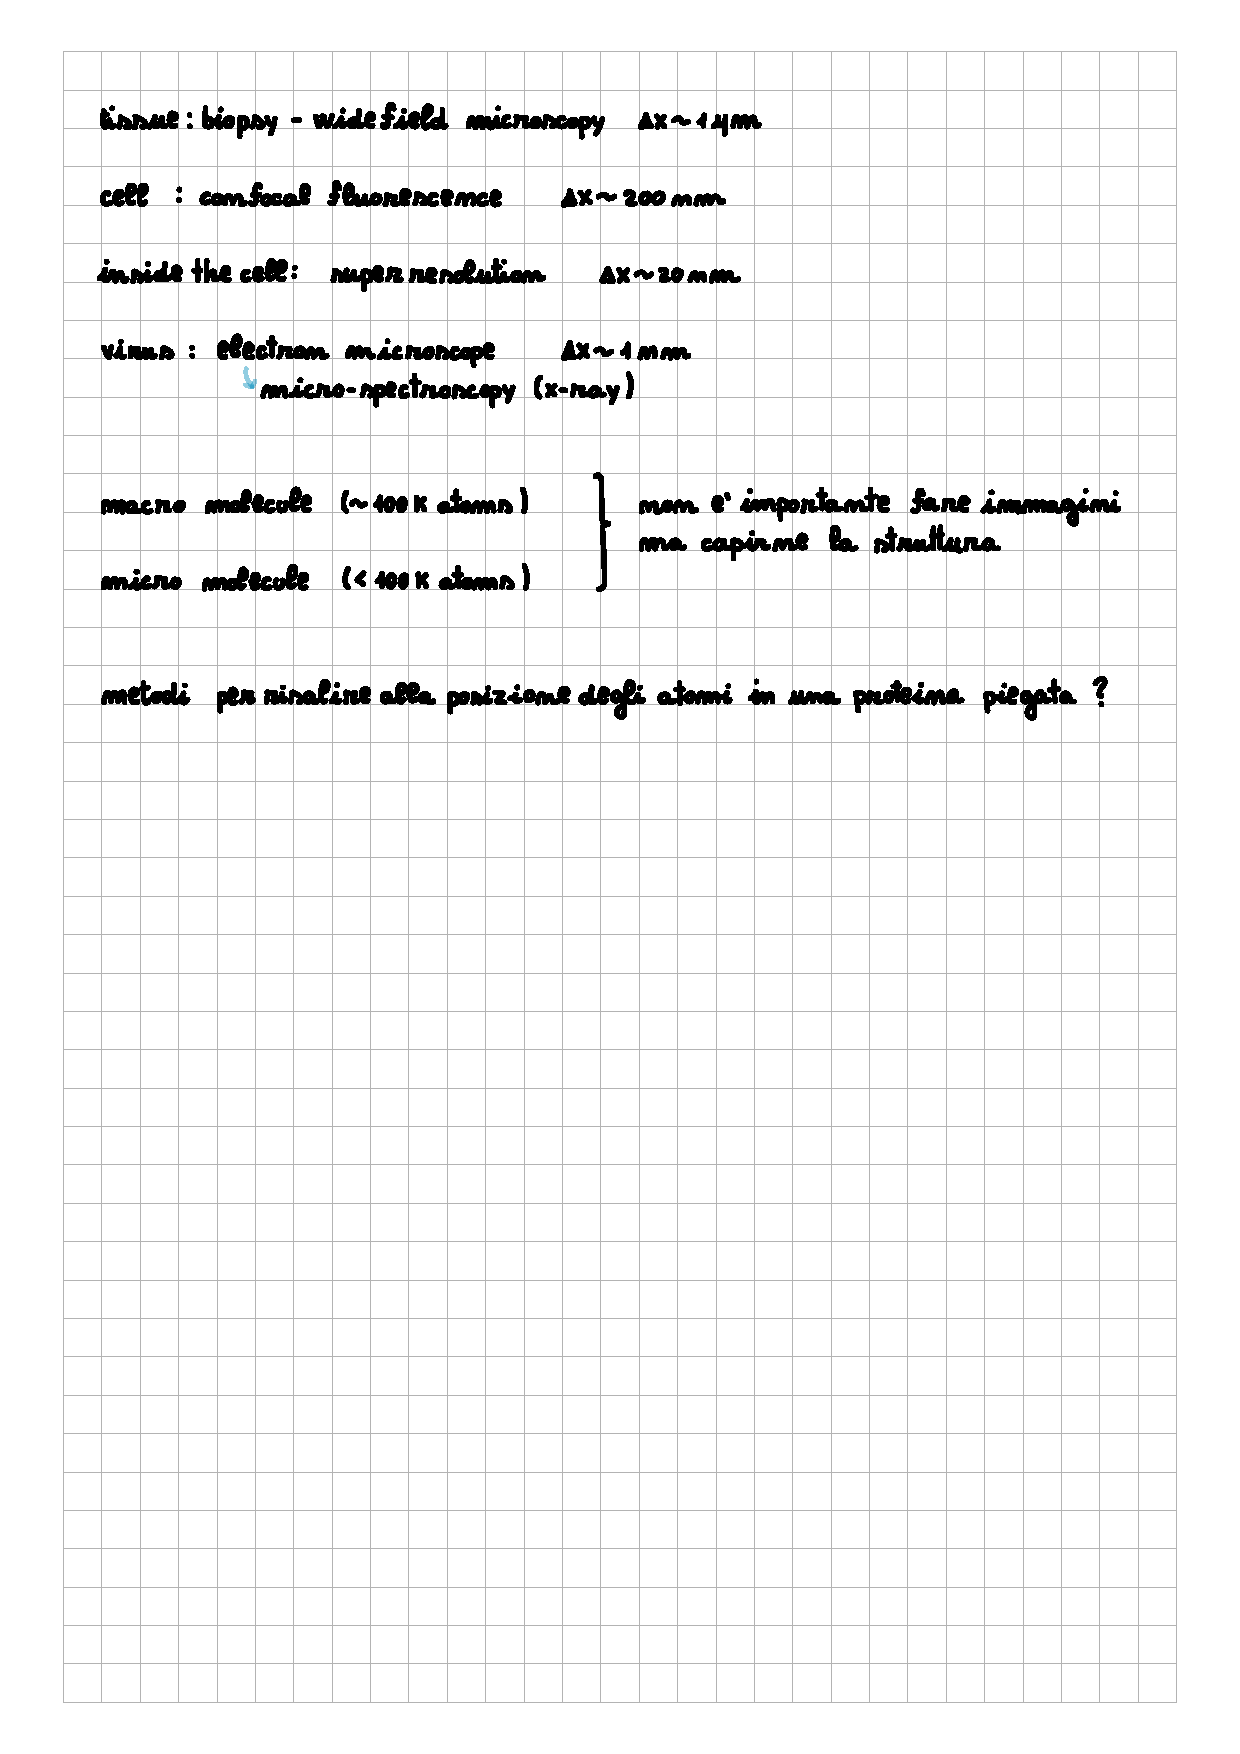
\includegraphics[width=\textwidth]{pics/04.png}
    \end{minipage}

    \begin{minipage}[b]{0.4\textwidth}
        \centering
        \includegraphics[width=\textwidth]{pics/05.png}
    \end{minipage}
    \caption{Andamento di $F(m)$ al variare della temperatura.}
    \label{fig:F(m)}
\end{figure}

